\documentclass[11pt]{article}
\renewcommand{\baselinestretch}{1.05}
\usepackage{amsmath,amsthm,verbatim,amssymb,amsfonts,amscd, graphicx}
\usepackage{blindtext}

\usepackage{caption}
\usepackage{enumitem}

%Additional Packages
\usepackage{enumitem}
\usepackage{graphics}
\usepackage{float}
\graphicspath{ {images/} }
%\usepackage[framed]{mcode}
\usepackage{hyperref}
\hypersetup{
	colorlinks=true,
	linkcolor=blue,
	filecolor=magenta,      
	urlcolor=cyan,
}

\topmargin0.0cm
\headheight0.0cm
\headsep0.0cm
\oddsidemargin0.0cm
\textheight23.0cm
\textwidth16.5cm
\footskip1.0cm
\theoremstyle{plain}
\newtheorem{theorem}{Theorem}
\newtheorem{corollary}{Corollary}
\newtheorem{lemma}{Lemma}
\newtheorem{proposition}{Proposition}
\newtheorem*{surfacecor}{Corollary 1}
\newtheorem{conjecture}{Conjecture} 
\newtheorem{question}{Question} 
\theoremstyle{definition}
\newtheorem{definition}{Definition}

\usepackage{indentfirst}
%\renewcommand{\thesubsubsection}{\thesubsection.\alph{subsection}}

\newcommand{\floor}[1]{\lfloor #1 \rfloor}

%SETUP PSUEDOCODE
\usepackage{tcolorbox}


%SETUP AtxMEGA128A1U
\usepackage{listings}

\usepackage{xcolor}
\definecolor{bluekeywords}{rgb}{0.13,0.13,1}
\definecolor{greencomments}{rgb}{0,0.5,0}
\definecolor{turqusnumbers}{rgb}{0.17,0.57,0.69}
\definecolor{redstrings}{rgb}{0.5,0,0}

\lstdefinelanguage{atxmega128a1u}{
	morekeywords={include, ,org, rjmp, CSEG, db, equ, DSEG, match, with, rec, open, module, namespace, type, of, member, and, for, in, do, begin, end, fun, function, try, mutable, if, then, else},
	keywordstyle=\color{bluekeywords},
	sensitive=false,
	morecomment=[l][\color{greencomments}]{;},
	morecomment=[s][\color{greencomments}]{{/*}{*/}},
	morestring=[b]",
	stringstyle=\color{redstrings}
}

\lstnewenvironment{asmlisting}{
	\lstset{
		frame=single,
		language=atxmega128a1u,
		basicstyle=\ttfamily,
		breaklines=true,
		columns=fullflexible
	}
}
{}
%
% START OF DOCUMENT
%
\begin{document}
\captionsetup[figure]{labelfont=bf} 

\title{Lab 3}
\author{\textbf{Michael Arboleda}\\Lab Section: 7F34}
\maketitle
%
% PRELAB QUESTIONS
%
\section*{b. Answers to all pre-lab questions}
\begin{enumerate}[label={\arabic*)},font={\color{red}\bfseries}]
	%
	%1
	%
	\item How many TC0 channels are necessary to control all three LEDs in the uPAD’s RGB LED?
	\\[0.8ex]
	\textbf{ANS:} .
	.
\end{enumerate}
%
% PROBLEMS ENCOUNTERED
%
\section*{c. Problems Encountered}
.
%
% FUTURE WORK
%
\section*{d. Future Work/Applications}
.
%
% SCHEMATICS
%
\section*{e. Schematics}
N/A
%
% PSEUDOCODE
%
\newpage
\section*{g. Pseudocode/Flowcharts}
%
% PSEUDOCODE PART B
%
\textbf{\textcolor{blue}{Pseudocode for lab1b.asm:}}
\begin{tcolorbox}
\begin{verbatim}
MAIN:

    * Equate numbers
    * Set registers to hold constants
    
    WHILE(true){
        * Grab data from buttons
        * AND Data with #4 to isolate 3rd bit 
        IF(S1 is pressed){
            * run subroutine display	
        }
        ELSE-IF(AND #8 to isolate4th bit 
          then check if S2 is pressed){
              * run subroutine fetch_store
        }
    }
END

SUBROUTINE DISPLAY:
    * Set PortC to be able write
    * Load LED data from memory
    * Display LEDs
    * Return to program

SUBROUTINE FETCH_STORE:
    * Set Port A to read
    * Read switches 
    * Store data in memory
    * Return to program
\end{verbatim}
\end{tcolorbox}
%
% PSEUDOCODE PART C
%
\newpage
\textbf{\textcolor{blue}{Pseudocode for lab1c.asm:}}
\begin{tcolorbox}
\begin{verbatim}
MAIN:

    * Equate numbers
    * Set registers to hold constants
    
    WHILE(true){
        * Set to write
        * Toggle LEDs off
        * Call DELAYx10ms subroutine
        * Toggle single LED on
        * Call DELAYx10ms subroutine
    }	
END


SUBROUTINE DELAY_10ms
    * Load number of iterations for loop as counter
    FOR( 
        Counter					;
        Counter does not equal 0	;
        Decrement interation by 1	
    )
    {No Body}
    * Return to program


SUBROUTINE DELAYx10ms
    * Parameter: multiplier to 10ms
    FOR(
        X := 0;
        X does not equal multiplier;
        Increment X by 1 
    )
    {
        * Call DELAY_10ms
    }	
    * Return to program	
\end{verbatim}
\end{tcolorbox}
%
% PSEUDOCODE PART D
%
\newpage
\textbf{\textcolor{blue}{Pseudocode for lab1d.asm:}}
\begin{tcolorbox}
\begin{verbatim}
MAIN:

    * Equate numbers
    * Set registers to hold constants
    
    WHILE(true){
        * Set pointer to KITT Table
        FOR(
            x := 0;
            x is not equal to table size;
            increment x by 1
        )
        {
            * LOAD table data
            * Increment z pointer
            
            * Turn LED on and Delay
            * Turn LED off and Delay
            * Turn LED on and Delay
            * Turn LED off and Delay
            * Turn LED on and Delay
        }
    }

END

SUBROUTINE DELAY_10ms
    * Load number of iterations for loop as counter
    FOR( 
        Counter					    ;
        Counter does not equal 0	;
        Decrement interation by 1	
        )
    {No Body}
    * Return to program	
\end{verbatim}
\end{tcolorbox}
\newpage
\section*{h. Program Code}
\textbf{\textcolor{blue}{Code for lab1b.asm:}}
\lstinputlisting[language=atxmega128a1u, frame=single]{lab1b.asm}
\textbf{\textcolor{blue}{Code for lab1c.asm:}}
\lstinputlisting[language=atxmega128a1u, frame=single]{lab1c.asm}
\textbf{\textcolor{blue}{Code for lab1d.asm:}}
\lstinputlisting[language=atxmega128a1u, frame=single]{lab1d.asm}
\section*{i. Appendix}
%\begin{figure}[H]
%	\centering
%	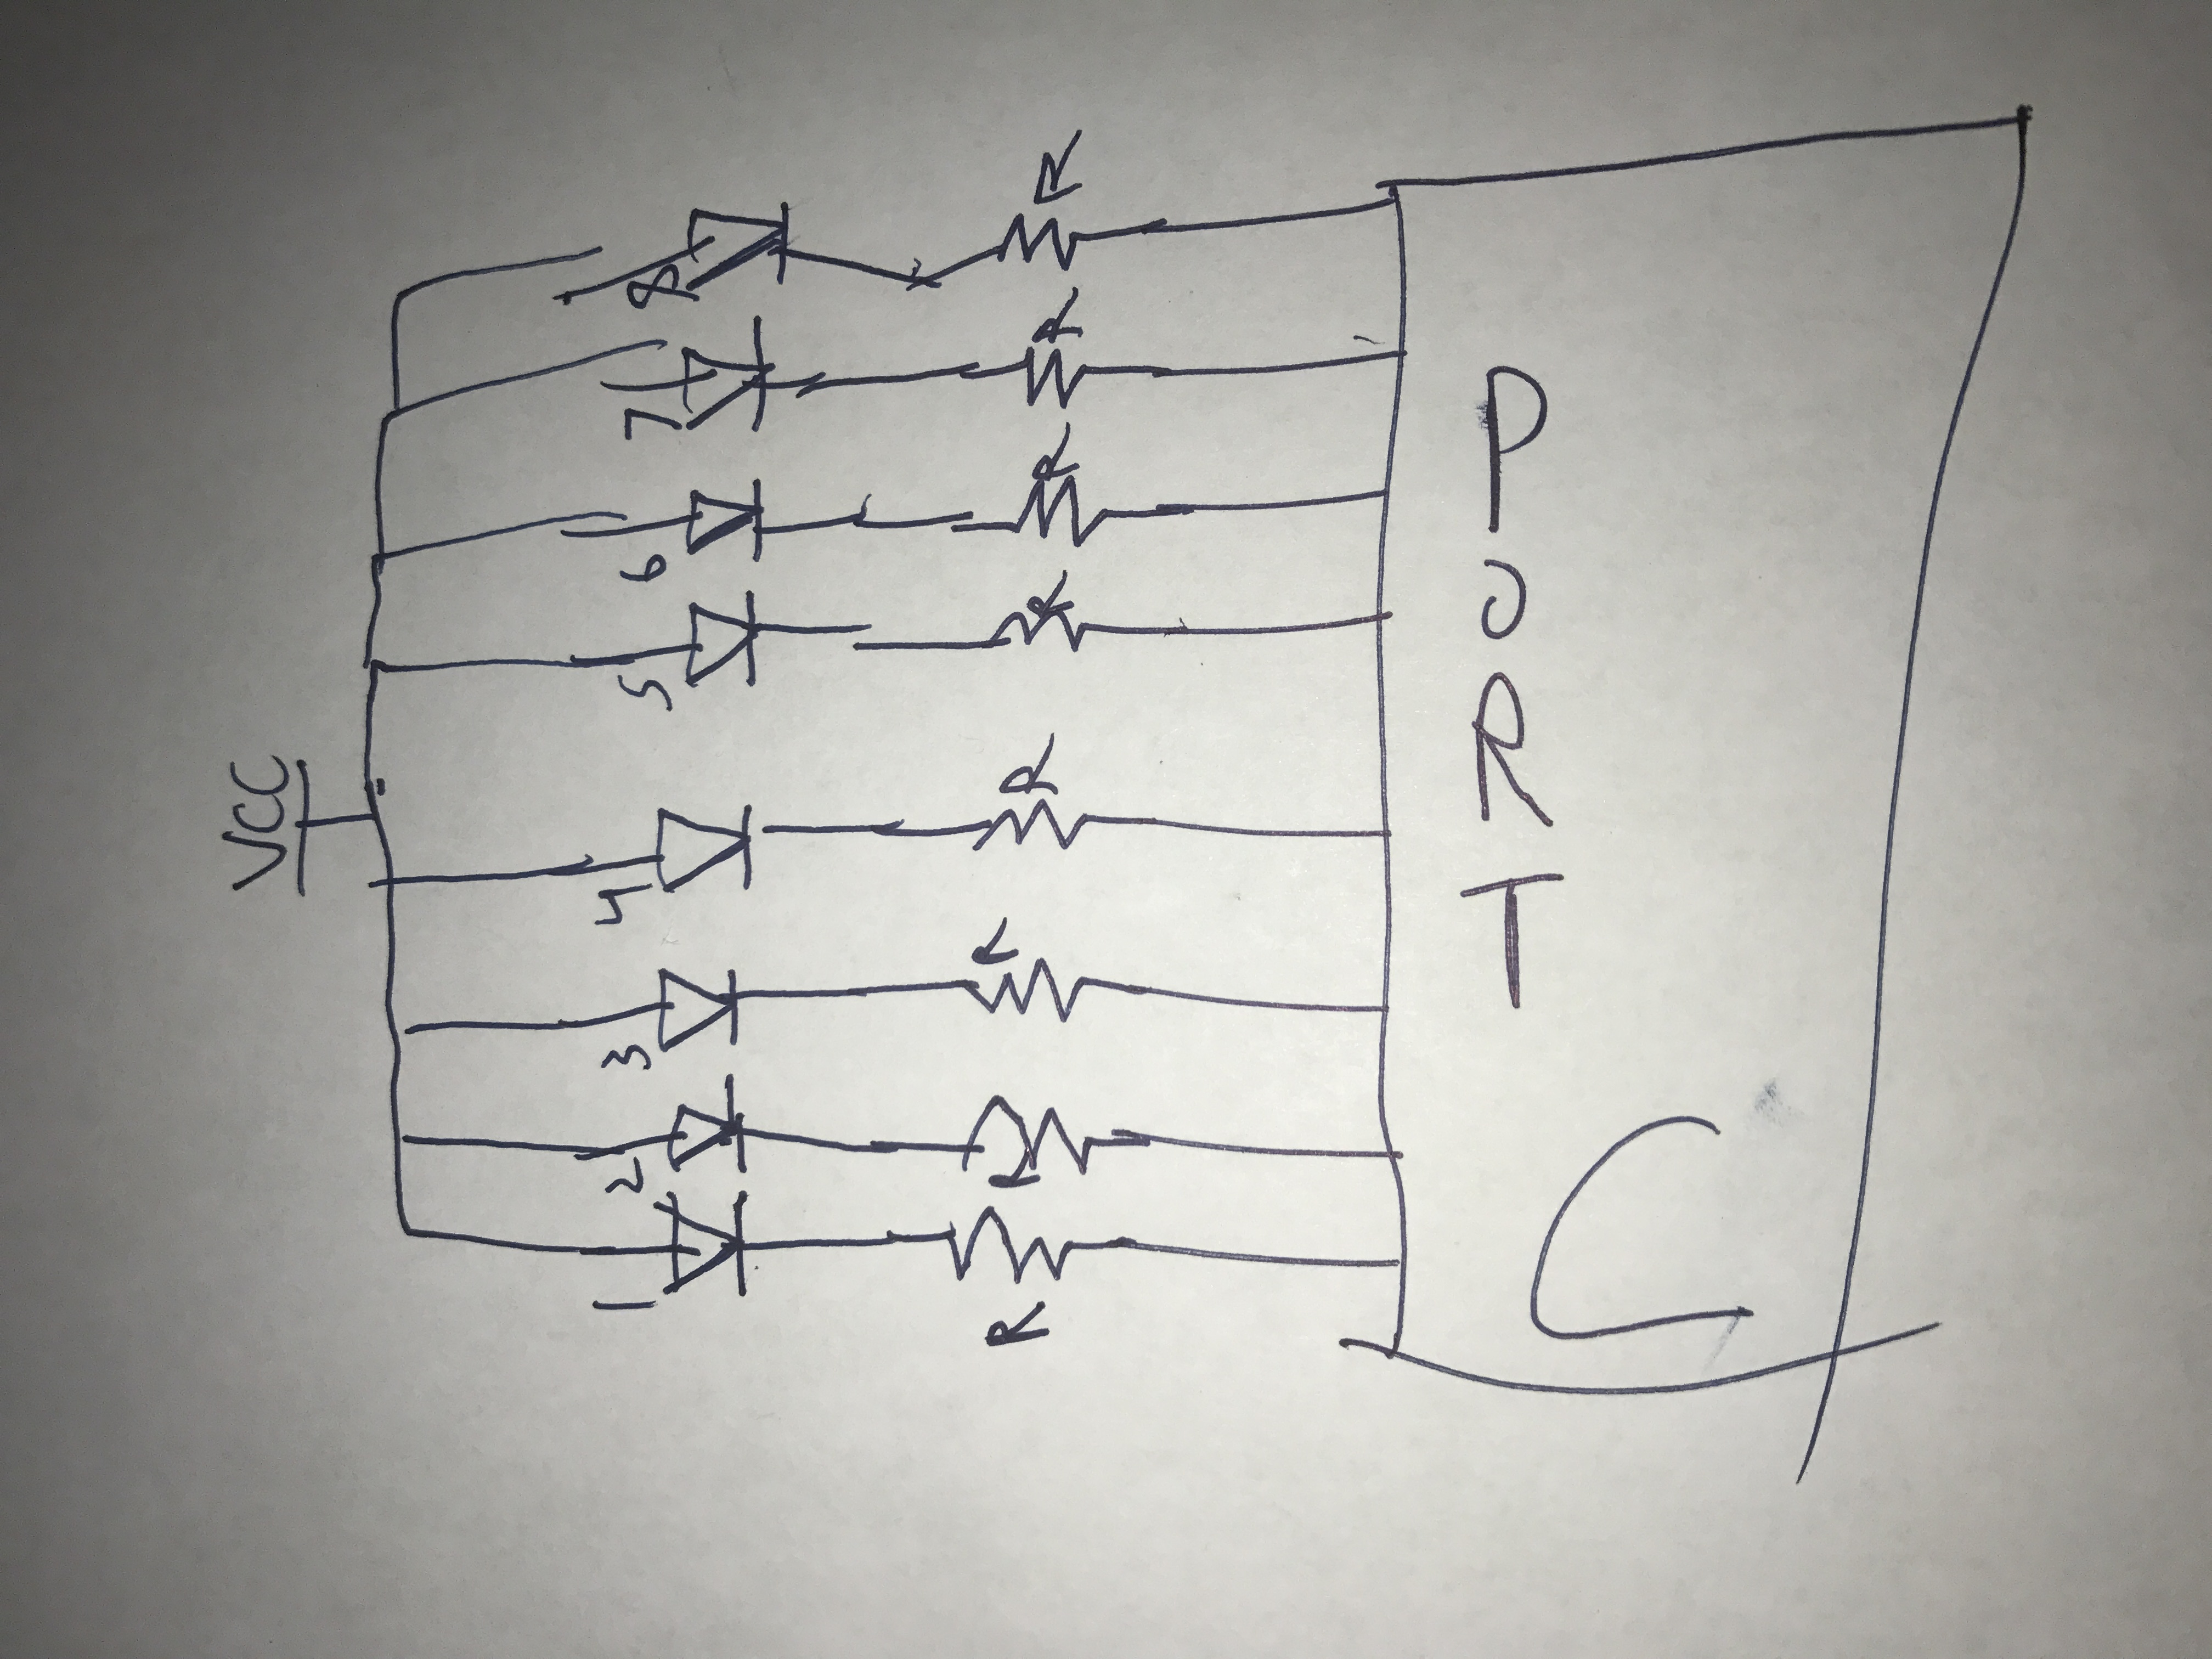
\includegraphics[width=\textwidth]{a}
%	\label{fig:c1}
%	\caption{PART A: LEDs wired to PORT C diagram}
%\end{figure}
\end{document}